

\tikzset{every picture/.style={line width=0.75pt}} %set default line width to 0.75pt        

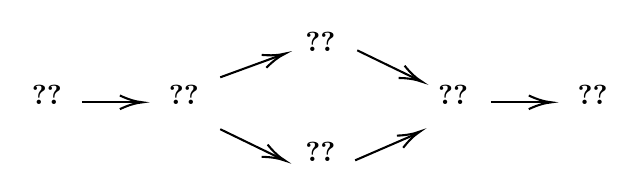
\begin{tikzpicture}[x=0.75pt,y=0.75pt,yscale=-1,xscale=1]
%uncomment if require: \path (0,82); %set diagram left start at 0, and has height of 82

%Straight Lines [id:da46646531768070965] 
\draw    (32.65,36.5) -- (59.88,36.5) ;
\draw [shift={(61.88,36.5)}, rotate = 180] [color={rgb, 255:red, 0; green, 0; blue, 0 }  ][line width=0.75]    (10.93,-3.29) .. controls (6.95,-1.4) and (3.31,-0.3) .. (0,0) .. controls (3.31,0.3) and (6.95,1.4) .. (10.93,3.29)   ;
%Straight Lines [id:da8027149644960445] 
\draw    (99.3,24.46) -- (128.8,13.68) ;
\draw [shift={(130.67,12.99)}, rotate = 159.93] [color={rgb, 255:red, 0; green, 0; blue, 0 }  ][line width=0.75]    (10.93,-3.29) .. controls (6.95,-1.4) and (3.31,-0.3) .. (0,0) .. controls (3.31,0.3) and (6.95,1.4) .. (10.93,3.29)   ;
%Straight Lines [id:da7707667943402254] 
\draw    (164.3,64.46) -- (193.8,51.68) ;
\draw [shift={(195.67,50.5)}, rotate = 152.93] [color={rgb, 255:red, 0; green, 0; blue, 0 }  ][line width=0.75]    (10.93,-3.29) .. controls (6.95,-1.4) and (3.31,-0.3) .. (0,0) .. controls (3.31,0.3) and (6.95,1.4) .. (10.93,3.29)   ;
%Straight Lines [id:da4813954173932613] 
\draw    (99.3,49.46) -- (128.72,63.72) ;
\draw [shift={(130.52,64.59)}, rotate = 205.86] [color={rgb, 255:red, 0; green, 0; blue, 0 }  ][line width=0.75]    (10.93,-3.29) .. controls (6.95,-1.4) and (3.31,-0.3) .. (0,0) .. controls (3.31,0.3) and (6.95,1.4) .. (10.93,3.29)   ;
%Straight Lines [id:da7934170316175215] 
\draw    (165.3,11.46) -- (194.72,25.72) ;
\draw [shift={(196.52,26.59)}, rotate = 205.86] [color={rgb, 255:red, 0; green, 0; blue, 0 }  ][line width=0.75]    (10.93,-3.29) .. controls (6.95,-1.4) and (3.31,-0.3) .. (0,0) .. controls (3.31,0.3) and (6.95,1.4) .. (10.93,3.29)   ;
%Straight Lines [id:da10093602464196261] 
\draw    (229.65,36.5) -- (256.88,36.5) ;
\draw [shift={(258.88,36.5)}, rotate = 180] [color={rgb, 255:red, 0; green, 0; blue, 0 }  ][line width=0.75]    (10.93,-3.29) .. controls (6.95,-1.4) and (3.31,-0.3) .. (0,0) .. controls (3.31,0.3) and (6.95,1.4) .. (10.93,3.29)   ;

% Text Node
\draw (7.02,26.8) node [anchor=north west][inner sep=0.75pt]    
{\ref{eq:ncsysP6}};
% Text Node
\draw (73.02,26.8) node [anchor=north west][inner sep=0.75pt]    
{\ref{eq:ncsysP5}};
% Text Node
\draw (138.8,1.04) node [anchor=north west][inner sep=0.75pt]   
{\ref{eq:ncsysP3'}};
% Text Node
\draw (138.8,54.4) node [anchor=north west][inner sep=0.75pt]    
{\ref{eq:ncsysP4}};
% Text Node
\draw (202.77,26.8) node [anchor=north west][inner sep=0.75pt]    
{\ref{eq:ncsysP2}};
% Text Node
\draw (270.02,26.8) node [anchor=north west][inner sep=0.75pt]    
{\ref{eq:ncsysP1}};


\end{tikzpicture}
